\chapter{Stetige  Funktionen}
\section{Motivation und Definition der Stetigkeit}
Wir wollen in diesem Abschnitt pr\"azisieren, wann eine Funktion so beschaffen ist, dass
wir sie zeichnen k\"onnen, ohne dabei den Stift absetzen zu m\"ussen.  F\"ur eine solche Funktion soll au{\ss}erdem der
\emph{Zwischenwert-Satz} gelten.  Der Zwischenwert-Satz besagt, dass f\"ur eine Funktion
\\[0.2cm]
\hspace*{1.3cm}
$f: \mathbb{R} \rightarrow \mathbb{R}$,
\\[0.2cm]
die wir ohne abzusetzen zeichnen k\"onnen, Folgendes gilt:
Falls es $a,b \in \mathbb{R}$ gibt mit $f(a) < 0$ und $f(b) > 0$, dann existiert auch ein $c \in\mathbb{R}$, 
so dass $f(c) = 0$ ist.  Anschaulich ist dieser Satz klar:  Ist beispielsweise $a < b$
und zeichne ich die Funktion $f$ in dem Intervall $[a, b]$, so muss der Graph der Funktion an irgendeiner
Stelle des Intervalls $[a,b]$ die $x$-Achse schneiden.  Voraussetzung daf\"ur, dass dies tats\"achlich so
ist, ist aber die Forderung, dass die Funktion $f$ keine Spr\"unge macht, denn wenn wir
beispielsweise die Funktion 
\\[0.2cm]
\hspace*{1.3cm}
$g: \mathbb{R} \rightarrow \mathbb{R}$
\\[0.2cm]
betrachten, die durch 
\\[0.2cm]
\hspace*{1.3cm}
$g(x) := \left\{
 \begin{array}{ll}
 -1 & \mbox{falls $x <    0$} \\ 
 +1 & \mbox{falls $x \geq 0$} \\ 
 \end{array}
 \right.
$
\\[0.2cm]
definiert ist, so haben wir zwar  $g(-1) = -1$ und $g(1) = 1$, aber es gibt kein $x \in [-1,1]$, 
f\"ur das $g(x) = 0$ w\"are.   Das liegt daran, dass die Funktion an der Stelle $x = 0$ einen Sprung
hat.  Unser Ziel in diesem Abschnitt ist es, zun\"achst exakt zu
definieren, was wir unter einer Funktion verstehen wollen, die keine Spr\"unge hat.  
In der Mathematik bezeichnen wir eine solche Funktion als  \colorbox{orange}{\emph{stetig}}.
Um den Begriff der \href{https://de.wikipedia.org/wiki/Stetigkeit}{Stetigkeit}
 einf\"uhren zu k\"onnen, bedarf es einer Reihe von zus\"atzlichen Definitionen, die nun folgen.

\begin{Definition}
Es sei $\folge{x_n}$ eine Folge und $D\subseteq \mathbb{R}$.  Wir sagen, dass 
\emph{die Folge $\folge{x_n}$ in $D$ liegt}, wenn f\"ur alle $n \in \mathbb{N}$ das Folgenglied $x_n
\in D$ ist.   
\end{Definition}

\begin{Definition}[Grenzwert einer Funktion]
  Es sei $D\subseteq \mathbb{R}$ und $f:D \rightarrow \mathbb{R}$.
  Weiter sei $\widehat{x} \in \mathbb{R}$ und  $\lambda\in \mathbb{R}$.  Au{\ss}erdem gebe es
  mindestens eine Folge $\folge{x_n}$, die gegen $\widehat{x}$ konvergiert.
  Dann ist $\lambda$ der \emph{Grenzwert} der Funktion $f$ \emph{im Punkt} $\widehat{x}$,
  wenn f\"ur jede in $D$ liegende Folge $\folge{x_n}$ gilt:
      \\[0.2cm]
      \hspace*{1.3cm}      
      $\lim\limits_{n\rightarrow\infty} x_n = \widehat{x} \;\Rightarrow\; \lim\limits_{n\rightarrow\infty} f(x_n) = \lambda$.
      \\[0.2cm]
      In diesem Fall schreiben wir 
      \\[0.2cm]
      \hspace*{1.3cm}      
      $\lim\limits_{x \rightarrow \widehat{x}} f(x) = \lambda$. 
      \eod
\end{Definition}

\noindent
\textbf{Bemerkung}:  In der obigen Definition ist nicht gefordert,
dass $\widehat{x}$ ein Element des Definitions-Bereichs  $D$ ist.  In vielen interessanten F\"allen
ist dies auch nicht der Fall, beispielsweise werden wir sp\"ater zeigen, dass 
\\[0.2cm]
\hspace*{1.3cm}      
$\lim\limits_{x \rightarrow 0} \bruch{\sin(x)}{x} = 1$
\\[0.2cm]
gilt. Die Funktion $x \mapsto \bruch{\sin(x)}{x}$ ist f\"ur $x=0$ nicht definiert, trotzdem
existiert der Grenzwert.
\eox


\begin{Definition}[Stetigkeit]
  Es sei $D\subseteq \mathbb{R}$ und $f:D \rightarrow \mathbb{R}$.
  Weiter sei $\widehat{x}\in D$. Dann ist die Funktion $f$ \emph{stetig im Punkt} $\widehat{x}$,
  wenn gilt: \\[0.2cm]
  \hspace*{1.3cm}      
  $\lim\limits_{x\rightarrow \widehat{x}} f(x) = f(\widehat{x})$.  \eod
\end{Definition}

\noindent
Aus den beiden letzten Definitionen folgt, dass
f\"ur eine stetige Funktion der Prozess der Grenzwert-Bildung mit der Anwendung der Funktion
vertauschbar ist.  F\"ur eine konvergente Folge $\folge{x_n}$ und eine stetige Funktion $f$ gilt 
      \\[0.2cm]
      \hspace*{1.3cm}      
      $f\Bigl(\lim\limits_{n\rightarrow\infty} x_n\Bigr) = \lim\limits_{n\rightarrow\infty} f(x_n)$.
\vspace*{0.3cm}

\noindent
\textbf{Beispiele}:
\begin{enumerate}
\item Es sei $c \in \mathbb{R}$.  Dann ist die konstante Funktion
      $f: \mathbb{R} \rightarrow \mathbb{R}$, die durch $f(x) := c$ definiert ist, in
      jedem Punkt $\widehat{x}\in\mathbb{R}$ stetig, denn f\"ur jede beliebige Folge $\folge{x_n}$ gilt 
      \\[0.2cm]
      \hspace*{1.3cm}      
      $\lim\limits_{n\rightarrow\infty} f(x_n) = \lim\limits_{n\rightarrow\infty} c = c$.
\item Die identische Funktion $\textsl{id}:\mathbb{R} \rightarrow \mathbb{R}$, die durch 
      $\textsl{id}(x) = x$ definiert ist, ist in jedem Punkt $\widehat{x}\in\mathbb{R}$ stetig,
      denn wenn $\folge{x_n}$ eine Folge ist, so dass
      \\[0.2cm]
      \hspace*{1.3cm}      
      $\lim\limits_{n\rightarrow\infty} x_n = \widehat{x}$
      \\[0.2cm]
      gilt, dann folgt sofort 
      \\[0.2cm]
      \hspace*{1.3cm}      
      $\lim\limits_{n\rightarrow\infty} \textsl{id}(x_n) = \lim\limits_{n\rightarrow\infty} x_n = \widehat{x}$.
\item Die Funktion $f: \mathbb{R} \rightarrow \mathbb{R}$, die durch
      $f(x) = x^2$ definiert ist, ist in jedem Punkt stetig, denn falls
      $\folge{x_n}$ eine Folge ist, so dass 
      \\[0.2cm]
      \hspace*{1.3cm}      
      $\lim\limits_{n\rightarrow\infty} x_n = \widehat{x}$ 
      \\[0.2cm]
      gilt, dann folgt nach dem Satz \"uber den Grenzwert einer Folge von Produkten
      \\[0.2cm]
      \hspace*{1.3cm}      
      $\lim\limits_{n\rightarrow\infty} f(x_n) = 
       \lim\limits_{n\rightarrow\infty} (x_n \cdot x_n) = 
       \left(\lim\limits_{n\rightarrow\infty} x_n\right) \cdot\left(\lim\limits_{n\rightarrow\infty} x_n\right) =
       \widehat{x} \cdot \widehat{x} = \widehat{x}^2$.
\item Das letzte Beispiel l\"asst sich verallgemeinern: Die Funktionen
      $f:\mathbb{R} \rightarrow \mathbb{R}$ und $g:\mathbb{R} \rightarrow \mathbb{R}$
      seien im Punkt $\widehat{x}$ stetig.  Dann ist auch die Funktion
      $h: \mathbb{R} \rightarrow \mathbb{R}$ die durch $h(x) := f(x) \cdot g(x)$
      definiert ist, stetig.  Denn sei $\folge{x_n}$ eine Folge, die gegen $\widehat{x}$
      konvergiert.  Dann gilt
      \\[0.2cm]
      \hspace*{1.3cm}      
      $
      \begin{array}[t]{lcll}
            \lim\limits_{n\rightarrow\infty} h(x_n) 
      & = & \lim\limits_{n\rightarrow\infty} f(x_n) \cdot g(x_n) & \mbox{Definition von $h$} \\[0.3cm] 
      & = & \left(\lim\limits_{n\rightarrow\infty} f(x_n)\right) \cdot \left(\lim\limits_{n\rightarrow\infty} g(x_n)\right) &
            \mbox{Grenzwert von Produkten} \\[0.3cm] 
      & = & f\left(\lim\limits_{n\rightarrow\infty} x_n\right) \cdot g\left(\lim\limits_{n\rightarrow\infty} x_n\right) &
            \mbox{$f$ und $g$ sind stetig} \\[0.3cm] 
      & = & f\bigr(\widehat{x}\bigr) \cdot g\bigr(\widehat{x}\bigr) &
            \lim\limits_{n\rightarrow\infty} x_n = \widehat{x} \\[0.3cm] 
      & = & h\bigl(\widehat{x}\bigr) & \mbox{Definition von $h$}
      \end{array}
      $
      
\item Mit einer zum letzten Fall analogen Argumentation k\"onnen wir leicht einsehen, dass alle Funktionen,
      die ausgehend von den konstanten Funktionen $x \mapsto c$ und der identischen
      Funktion $x \mapsto x$ mit Hilfe der elementaren Rechen-Operationen 
      ``$+$'', ``$-$'', ``$\cdot $'' und ``$/$'' gebildet werden k\"onnen, stetig sind.  Solche
      Funktionen werden als \href{http://de.wikipedia.org/wiki/Rationale_Funktion}{\emph{rationale Funktionen}} bezeichnet.
      Ein       Beispiel f\"ur eine solche Funktion ist 
      \\[0.2cm]
      \hspace*{1.3cm}      
      $x \mapsto \bruch{x^3 - 2\cdot x +1}{x^2 -1}$.
      \\[0.2cm]
      Diese Funktion ist f\"ur alle $x\in\mathbb{R} \backslash \{1,-1\}$ definiert und ist
      nach der obigen Argumentation stetig.


\item Die Funktion $\textsl{sign}:\mathbb{R} \rightarrow \mathbb{R}$ sei durch
      \\[0.2cm]
      \hspace*{1.3cm}      
      $\textsl{sign}(x) = \left\{
       \begin{array}{rl}
        +1 & \mbox{falls}\; x > 0, \\
         0 & \mbox{falls}\; x = 0, \\
        -1 & \mbox{falls}\; x < 0. \\
       \end{array}\right.
      $
      \\[0.2cm]
      definiert. Diese Funktion ist im Punkt $0$ nicht stetig, denn f\"ur die Folge
      $\folge{\frac{1}{n}}$ gilt
      \\[0.2cm]
      \hspace*{1.3cm}      
      $\ds \lim\limits_{n\rightarrow\infty} \frac{1}{n} = 0$, \quad aber \quad
      $\ds \lim\limits_{n\rightarrow\infty} \textsl{sign}\left(\frac{1}{n}\right) =
       \lim\limits_{n\rightarrow\infty} 1 = 1 \not= 0 = \textsl{sign}(0)$. 

       Anschaulich ist die Funktion $\textsl{sign}:\mathbb{R} \rightarrow \mathbb{R}$  im Punkt
       0 nicht stetig, weil sie an dieser Stelle einen Sprung hat.
       \eox
\end{enumerate}

\begin{Definition}[Uneigentliche Konvergenz]
Wir sagen, dass eine Folge  $\folge{x_n}$ gegen Unendlich konvergiert und schreiben 
\\[0.2cm]
\hspace*{1.3cm}      
$\lim\limits_{n\rightarrow\infty} x_n = \infty$
\\[0.2cm]
wenn gilt:
\\[0.2cm]
\hspace*{1.3cm}      
$\forall c \in \mathbb{R}: \exists K \in \mathbb{N}: \forall n \in \mathbb{N}: \bigl(n \geq K \rightarrow x_n > c\bigr)$.
\eod
\end{Definition}

\example  
F\"ur die Folge $\folge{n}$ gilt offenbar 
\\[0.2cm]
\hspace*{1.3cm}      
$\lim\limits_{n\rightarrow\infty} n = \infty$.
\eox

\begin{Definition}
Es sei $f:\mathbb{R} \rightarrow \mathbb{R}$ eine Funktion und $\lambda\in \mathbb{R}$.
Gilt f\"ur jede Folge $\folge{x_n}$
\\[0.2cm]
\hspace*{1.3cm}      
$\lim\limits_{n\rightarrow\infty} x_n = \infty \;\Rightarrow\;
     \lim\limits_{n\rightarrow\infty} f(x_n) = \lambda$,
\\[0.2cm]
dann schreiben wir 
\\[0.2cm]
\hspace*{1.3cm}      
$\lim\limits_{x\rightarrow\infty} f(x) = \lambda$.
\eod
\end{Definition}

\example 
Es gilt
\\[0.2cm]
\hspace*{1.3cm}      
$\lim\limits_{x\rightarrow\infty} \bruch{1}{x} = 0$.
\\[0.2cm]
\textbf{Beweis}:  Es sei eine Folge $\folge{x_n}$ gegeben, so dass 
\\[0.2cm]
\hspace*{1.3cm}      
$\lim\limits_{n\rightarrow\infty} x_n = \infty$
\\[0.2cm]
gilt.   Nach Definition der uneigentlichen Konvergenz gegen $\infty$ gilt dann
\begin{equation}
  \label{eq:stetig0}  
  \forall c \in \mathbb{R}: \exists K \in \mathbb{N}:\bigl(\forall n \in \mathbb{N}: n \geq K \rightarrow x_n > c\bigr)
\end{equation}
Wir m\"ussen zeigen, dass gilt:
\\[0.2cm]
\hspace*{1.3cm}
$\ds \lim\limits_{n\rightarrow\infty} \bruch{1}{x_n} = 0$.
\\[0.2cm]
Dies ist nach der Definition des Grenzwerts einer Folge \"aquivalent zu der Formel
\begin{equation}
  \label{eq:stetig1}
  \forall \varepsilon \in\mathbb{R}_+: \exists K \in \mathbb{R} : \forall n \in \mathbb{N}
  :\Bigl(n \geq K \rightarrow \left|\frac{1}{x_n}\right| < \varepsilon\Bigr)
\end{equation}
Um diese Formel nachzuweisen, nehmen wir an, dass eine Zahl $\varepsilon>0$
gegeben ist.  Wir m\"ussen dann ein $K$ finden, so dass f\"ur alle nat\"urlichen Zahlen $n$, die
gr\"o{\ss}er-gleich $K$ sind, die Ungleichung 
\\[0.2cm]
\hspace*{1.3cm} $\left|\bruch{1}{x_n}\right| < \varepsilon$
\\[0.2cm]
gilt.  Dies gelingt uns mit Hilfe der Formel (\ref{eq:stetig0}), denn wenn wir in dieser Formel
$\ds c := \frac{1}{\varepsilon}$ definieren, dann finden wir eine Zahl $K$, so dass f\"ur alle
nat\"urlichen Zahlen $n$, die
gr\"o{\ss}er-gleich $K$ sind, die Ungleichung  
\\[0.2cm] \hspace*{1.3cm} $\displaystyle x_n > c$, \quad also $\displaystyle x_n > \frac{1}{\varepsilon}$ \\[0.2cm]
gilt.  Invertieren wir nun diese Ungleichung, so folgt
\\[0.2cm]
\hspace*{1.3cm}
$\bruch{1}{x_n} < \varepsilon$
\\[0.2cm]
und da andererseits aus $x_n > \frac{1}{\varepsilon}$ und $\varepsilon > 0$ auch $x_n > 0$
und damit $\bruch{1}{x_n} > 0$ folgt, haben wir insgesamt 
\\[0.2cm]
\hspace*{1.3cm}
$\left|\bruch{1}{x_n}\right| < \varepsilon$
\\[0.2cm]
f\"ur alle $n \geq K$ gezeigt. \hspace*{\fill} $\Box$
\vspace*{0.3cm}

\noindent
Es gibt eine alternative Definition der Stetigkeit, die zu der oben gegebenen Definition
\"aquivalent ist. Diese Definition tr\"agt den Namen 
\href{http://de.wikipedia.org/wiki/Epsilon-Delta-Kriterium#Stetigkeit_reeller_Funktionen}{\emph{$\varepsilon$-$\delta$-Definition der Stetigkeit}} 
und Funktionen, die nach dieser Definition stetig sind, hei{\ss}en $\varepsilon$-$\delta$-stetig.

\begin{Definition}[$\varepsilon$-$\delta$-Stetigkeit] 
  Eine Funktion $f:D \rightarrow \mathbb{R}$ ist \colorbox{orange}{\emph{$\varepsilon$-$\delta$-stetig}} im Punkt
  $\widehat{x}$, wenn gilt: 
  \\[0.2cm]
  \hspace*{1.3cm}
  $\forall \varepsilon \in \mathbb{R}_+: \exists \delta \in \mathbb{R}_+: \forall x \in D: 
   \bigl(|x - \widehat{x}| < \delta \rightarrow |f(x) - f(\widehat{x})| < \varepsilon\bigr)$.
  \eod
\end{Definition}


\exercise
\begin{enumerate}[(a)]
\item Zeigen Sie, dass jede Funktion, die $\varepsilon$-$\delta$-stetig ist,
      auch stetig ist.
\item Zeigen Sie, dass jede stetige Funktion auch $\varepsilon$-$\delta$-stetig ist.

      \hint 
      F\"uhren Sie den Beweis von Teil (b) dieser Aufgabe indirekt.
      \eox
\end{enumerate}


\begin{Definition}[Allgemeine Stetigkeit] \lb
Eine Funktion $f:D \rightarrow \mathbb{R}$ hei{\ss}t \colorbox{orange}{\emph{stetig}} genau dann, wenn
die Funktion $f$ f\"ur alle $\widehat{x} \in D$ stetig ist.
\eod
\end{Definition}

\exercise
Es sei $f: \mathbb{R} \rightarrow \mathbb{R}$.  Geben Sie eine sinnvolle Definition f\"ur 
\\[0.2cm]
\hspace*{1.3cm}
$\lim\limits_{x\rightarrow\infty} f(x) = \infty$.
\eox

\remark
Wir haben den Begriff des Grenzwerts einer Funktion mit Hilfe von Folgen definiert.  Es gibt eine
dazu \"aquivalente $\varepsilon$-$\delta$-Definition des Grenzwerts.  Bei dieser Definition sagen wir,
dass eine Funktion
\\[0.2cm]
\hspace*{1.3cm}
$f: D \rightarrow \mathbb{R}$
\\[0.2cm]
an der Stelle $\bar{x}$ den Grenzwert $\lambda$ hat, wenn
\\[0.2cm]
\hspace*{1.3cm}
$\forall \varepsilon\in\mathbb{R}_+: \exists\delta\in\mathbb{R}_+: \forall x\in D:\bigl(|x-\bar{x}|<\delta \rightarrow |f(x) - \lambda| < \varepsilon\bigr)$
\\[0.2cm]
gilt.  Genau wie die $\varepsilon$-$\delta$ Definition der Stetigkeit \"aquivalent ist zu dem
Stetigkeits-Begriff, den wir mit Hilfe von Folgen definiert haben, ist auch die
$\varepsilon$-$\delta$-Definition des Grenzwerts \"aquivalent zu der Definition des
\href{http://de.wikipedia.org/wiki/Grenzwert_(Funktion)}{Grenzwerts}, die wir 
fr\"uher mit Hilfe von Folgen gegeben haben.  Der Beweis dieser Behauptung ist Gegenstand der 
folgenden Aufgabe.
\pagebreak

\exercise
Es sei \\[0.2cm]
\hspace*{1.3cm}
$f: D \rightarrow \mathbb{R}$
\\[0.2cm]
eine reellwertige Funktion.  Beweisen Sie die beiden folgenden Behauptungen:
\begin{enumerate}[(a)]
\item Falls die Formel
      \\[0.2cm]
      \hspace*{1.3cm}
      $\forall \varepsilon\in\mathbb{R}_+: \exists\delta\in\mathbb{R}_+: \forall x\in D:\bigl(|x-\bar{x}|<\delta \rightarrow |f(x) - \lambda| < \varepsilon\bigr)$
      \\[0.2cm]
      richtig ist, dann gilt
      $\ds \lim\limits_{x\rightarrow\bar{x}} f(x) = \lambda$.
\item Falls  $\ds \lim\limits_{x\rightarrow\bar{x}} f(x) = \lambda$ gilt, dann gilt auch
      \\[0.2cm]
      \hspace*{1.3cm}
      $\forall \varepsilon\in\mathbb{R}_+: \exists\delta\in\mathbb{R}_+: \forall x\in D:\bigl(|x-\bar{x}|<\delta \rightarrow |f(x) - \lambda| < \varepsilon\bigr)$.
      \eox
\end{enumerate}



\section{Bestimmung von Nullstellen}
In der Praxis tritt h\"aufig die Frage auf, ob eine Funktion in einem bestimmten Intervall
eine Nullstelle hat.  Zus\"atzlich werden Verfahren ben\"otigt, mit denen eine solche
Nullstelle gegebenenfalls berechnet werden kann.

\begin{Satz}[Zwischenwert-Satz] \label{satz:zws-stetig}
Die Funktion $f:[a,b] \rightarrow \mathbb{R}$ sei stetig.  Weiter sei $f(a) \leq 0$ und
$f(b) \geq 0$.  Dann gibt es ein $x_0 \in [a,b]$, so dass $f(x_0) = 0$ ist.
\end{Satz}

\noindent
\textbf{Beweis}: Wir geben ein Verfahren an, mit dem eine Nullstelle berechnet werden kann
und weisen dann nach, dass der von diesem Verfahren gelieferte Wert tats\"achlich eine
Nullstelle der Funktion ist.  Das Verfahren, dass wir vorstellen werden, wird in der
Literatur als \emph{Verfahren der Intervall-Halbierung} oder auch als
\href{http://en.wikipedia.org/wiki/Bisection_method}{\emph{Bisektions-Verfahren}} bezeichnet.  
Das Verfahren folgt dem Paradigma ``\emph{Teile und Herrsche}''.  Im Englischen werden solche
Verfahren als
``\href{http://en.wikipedia.org/wiki/Divide_and_conquer_algorithms}{\emph{divide and conquer algorithms}}''
bezeichnet.
Beim Bisektions-Verfahren definieren wir induktiv zwei Folgen $\folge{a_n}$ und
$\folge{b_n}$ wie folgt:
\begin{enumerate}
\item[I.A.:] $n=1$.

      $a_1 := a$,  \quad $b_1 := b$.
\item[I.S.:] $n \mapsto n+1$

      Zun\"achst definieren wir $c_n$ als das arithmetische Mittel von $a_n$ und $b_n$:
      \\[0.2cm]
      \hspace*{1.3cm} $\ds c_n := \frac{1}{2} \cdot (a_n + b_n)$. \\[0.2cm]
      Dann definieren wir $a_{n+1}$ und $b_{n+1}$ simultan durch Fall-Unterscheidung:
      \\[0.2cm]
      \hspace*{1.3cm}
      $\pair(a_{n+1}, b_{n+1}) := \left\{ \begin{array}{ll}
                          \pair(a_n,c_n) & \mbox{falls}\quad f(c_n) >    0 \\
                          \pair(c_n,b_n)   & \mbox{falls}\quad f(c_n) \leq 0. \\
                          \end{array}
                  \right.
      $
\end{enumerate}
Aus dieser Definition folgt sofort per Induktion, dass f\"ur alle $n\in\mathbb{N}$
gilt:
\begin{enumerate}
\item $f(a_n) \leq 0$.
\item $f(b_n) \geq 0$.
\item $a_n \leq a_{n+1}$, \quad die Folge $\folge{a_n}$ ist also monoton
      steigend.
\item $b_n \geq b_{n+1}$, \quad die Folge $\folge{b_n}$ ist also monoton
      fallend.
\item $a_n \leq b_n$.
\item $\displaystyle b_n - a_n = \left(\frac{1}{2}\right)^{n-1} \cdot (b - a)$.
\end{enumerate}
Wir f\"uhren hier nur den Nachweis der letzten Behauptung vor, denn diese Behauptung
ist am wenigsten offensichtlich.
\begin{enumerate}
\item[I.A.:] $n = 1$. Es gilt 
      \\[0.2cm]
      \hspace*{1.3cm}
      $\ds b_1 - a_1 = b - a = \left(\frac{1}{2}\right)^{1-1} \cdot (b-a)$.
\item[I.S.:] $n \mapsto n+1$.  

      Es ist $\ds c_n = \frac{1}{2} \cdot (a_n + b_n)$.   Wir f\"uhren eine 
      Fall-Unterscheidung nach dem Vorzeichen von $f(c_n)$ durch.
      \begin{enumerate}
      \item $f(c_n) > 0$.  Dann gilt $a_{n+1} = a_n$ und 
            $\ds b_{n+1} = c_n = \frac{1}{2} \cdot(a_n + b_n)$.
            Also haben wir      
            \\[0.2cm]
            \hspace*{1.3cm}
            $
            \begin{array}[b]{lcl}
              b_{n+1} - a_{n+1} & = & \ds\frac{1}{2}\cdot(a_n + b_n) - a_n \\[0.4cm]
                               & = & \ds\frac{1}{2}\cdot(b_n - a_n)       \\[0.4cm]  
                  & \stackrel{IV}{=} & \ds\frac{1}{2}\cdot\left(\frac{1}{2}\right)^{n-1}\cdot(b - a) \\[0.4cm]  
                                & = & \ds\left(\frac{1}{2}\right)^{(n+1) - 1}\cdot(b - a) 
            \end{array}
            $$\surd$
      \item $f(c_n) \leq 0$.  Jetzt gilt $\ds a_{n+1} = c_n = \frac{1}{2}\cdot(a_n + b_n)$ und 
            $b_{n+1} = b_n$.
            Also haben wir      
            \\[0.2cm]
            \hspace*{1.3cm}
            $
            \begin{array}[b]{lcl}
              b_{n+1} - a_{n+1} & = & \ds b_n - \frac{1}{2}\cdot(a_n + b_n) \\[0.4cm]
                                & = & \ds\frac{1}{2}\cdot(b_n - a_n)       \\[0.4cm]  
                  & \stackrel{IV}{=} & \ds\frac{1}{2}\cdot\left(\frac{1}{2}\right)^{n-1}\cdot(b - a) \\[0.4cm]  
                                & = & \ds\left(\frac{1}{2}\right)^{(n+1)-1}\cdot(b - a) 
            \end{array}
            $ $\surd$
      \end{enumerate}
      Damit ist die Behauptung in beiden F\"allen bewiesen.
\end{enumerate}
Aus den Behauptungen 3., 4., und 5.~folgt, dass die Folge $\folge{b_n}$ durch $a$ nach unten
beschr\"ankt ist, denn es gilt
\\[0.2cm]
\hspace*{1.3cm} $a = a_1 \leq \cdots \leq a_{n-1} \leq a_n \leq b_n$, \quad
                also gilt $a \leq b_n$ f\"ur alle $n\in\mathbb{N}$.
 \\[0.2cm]
Da die Folge $\folge{b_n}$ monoton fallend und nach unten beschr\"ankt ist, muss diese Folge
nach Satz \ref{satz:monoton} auch konvergent sein.  Wir definieren
\\[0.2cm]
\hspace*{1.3cm}
$\widehat{b} := \lim\limits_{n\rightarrow\infty} b_n$.
\\[0.2cm]
In analoger Weise sehen wir, dass die Folge $\folge{a_n}$ monoton steigend und nach oben
beschr\"ankt ist.  Also ist diese Folge ebenfalls konvergent und wir definieren
\\[0.2cm]
\hspace*{1.3cm}
$\widehat{a} := \lim\limits_{n\rightarrow\infty} a_n$.
\\[0.2cm]
Als n\"achstes weisen wir nach, dass $\widehat{a} = \widehat{b}$ ist.  Dazu betrachten wir
die Differenz der Grenzwerte: 
\\[0.2cm]
\hspace*{1.3cm}
$
\begin{array}[t]{lcl}  
\widehat{b} - \widehat{a} & = &
 \ds\left(\lim\limits_{n\rightarrow\infty} b_n\right) - \left(\lim\limits_{n\rightarrow\infty} a_n\right) \\[0.3cm]
& = & \ds\lim\limits_{n\rightarrow\infty} b_n - a_n \\[0.3cm]
& = & \ds\lim\limits_{n\rightarrow\infty} \left(\frac{1}{2}\right)^{n-1} \cdot (b-a) \\[0.3cm]
& = & \ds (b-a) \cdot \lim\limits_{n\rightarrow\infty} \left(\frac{1}{2}\right)^{n-1} = 0,
\end{array}
$
\\[0.2cm]
also gilt $\widehat{b} = \widehat{a}$. Da die Funktion $f$ stetig ist, gilt
\\[0.2cm]
\hspace*{1.3cm}
$\lim\limits_{n\rightarrow\infty} f(a_n) = f\left(\lim\limits_{n\rightarrow\infty} a_n\right) = f(\widehat{a})$.
\\[0.31cm]
Weil $f(a_n) \leq 0$ ist f\"ur alle $n\in\mathbb{N}$ folgt dann sofort
\\[0.2cm]
\hspace*{1.3cm}
$f(\widehat{a}) \leq 0$.
\\[0.2cm]
Genauso folgt aus der Stetigkeit von $f$, dass
\\[0.2cm]
\hspace*{1.3cm}
$\lim\limits_{n\rightarrow\infty} f(b_n) = f\left(\lim\limits_{n\rightarrow\infty}
  b_n\right) = f\bigl(\,\widehat{b}\,\bigr)$ 
\\[0.3cm]
gilt.  Aus $\forall n\in\mathbb{N}: f(b_n) \geq 0$ folgt dann sofort
\\[0.2cm]
\hspace*{1.3cm}
$f(\widehat{b}) \geq 0$.
\\[0.2cm]
Da $\widehat{a} = \widehat{b}$ gilt, haben wir nat\"urlich auch 
$f\bigl(\widehat{a}\bigr) = f\bigl(\,\widehat{b}\,\bigr)$.  Dann haben wir aber sowohl
\\[0.2cm]
\hspace*{1.3cm}
$f\bigl(\widehat{a}\bigr) \leq 0$ \quad als auch \quad $f\bigl(\widehat{a}\bigr) \geq 0$ 
\\[0.2cm]
und das funktioniert nur, wenn $f\bigl(\widehat{a}\bigr) = 0$ ist.  Damit k\"onnen wir $x_0 =
\widehat{a}$ definieren und dann ist $x_0$ eine
Nullstelle von $f$ in dem Intervall $[a,b]$.
\qed

\remark
In der Literatur finden Sie eine etwas allgemeinere Version des Zwischenwert-Satzes: Falls
\\[0.2cm]
\hspace*{1.3cm}
$f:[a,b] \rightarrow \mathbb{R}$
\\[0.2cm]  
eine stetige Funktion ist, so nimmt die Funktion jeden Wert zwischen den Werten $f(a)$ und $f(b)$ an.
Ist beispielsweise $f(a) < f(b)$, so gilt also
\\[0.2cm]
\hspace*{1.3cm}
$\forall c \in [f(a), f(b)]: \exists \bar{x} \in [a,b]: f(\bar{x}) = c$.
\\[0.2cm]
Dieser Satz l\"asst sich beweisen, indem wir die Funktion $g$ als
\\[0.2cm]
\hspace*{1.3cm}
$g := \bigl(x \mapsto f(x) - c\bigr)$
\\[0.2cm]
definieren.  Dann haben wir
\\[0.2cm]
\hspace*{1.3cm}
$g(a) = f(a) - c \leq 0$ \quad und \quad $g(b) = f(b) - c \geq 0$
\\[0.2cm]
und wir k\"onnen auf die Funktion $g$ den von uns bewiesen Zwischenwert-Satz anwenden.  Damit finden
eine Zahl $\bar{x} \in [a,b]$, f\"ur die $g(\bar{x}) = 0$ gilt.  Also haben wir
\\[0.2cm]
\hspace*{1.3cm}
$f(\bar{x}) -c = 0$
\\[0.2cm]
und daraus folgt $f(\bar{x}) = c$.  \eox

\exercise
\begin{enumerate}[(a)]
\item Die Funktion $f:[0,1] \rightarrow [0,1]$ sei stetig.  Zeigen Sie, dass die Funktion $f$ dann
      einen Fixpunkt hat, zeigen Sie also, dass es ein $x_0 \in [0,1]$ gibt, so dass
      \\[0.2cm]
      \hspace*{1.3cm}
      $f(x_0) = x_0$ \quad gilt.
      \pagebreak

\item Zeigen Sie, dass die Funktion $f: \mathbb{R} \rightarrow \mathbb{R}$, die durch $f(x) := \cos(x)$
      definiert ist, einen Fixpunkt hat.  Sie d\"urfen bei Ihrem Beweis voraussetzen, das die
      Funktion $x \mapsto \cos(x)$ stetig ist.  Au{\ss}erdem ist bekannt , dass diese Funktion im Intervall 
      $[0, \pi]$ monoton fallend ist.
      \eox
\end{enumerate}

\exercise
Es war einmal ein buddhistischer M\"onch, der einmal im Jahr zur Meditation auf einen Berg stieg.
Er begann seinen Weg um 6:00 Uhr morgens und erreichte den Gipfel um 18:00 Uhr abends.  Nachdem er
die ganze Nacht meditiert hatte, begann er am n\"achsten Morgen um 6:00 mit dem Abstieg, der bis 18:00
abends dauerte.  Beim Abstieg nahm der M\"onch den selben Weg wie beim Aufstieg.  Zeigen Sie, dass es
eine Tageszeit $t$ gibt, an welcher der M\"onch beim Abstieg am selben Ort ist wie beim Aufstieg. 
\eox
 
\subsection{Implementierung des Intervall-Halbierungs-Verfahrens}

\begin{figure}[!ht]
  \centering
\begin{Verbatim}[ frame         = lines, 
                  framesep      = 0.3cm, 
                  labelposition = bottomline,
                  numbers       = left,
                  numbersep     = -0.2cm,
                  xleftmargin   = 0.5cm,
                  xrightmargin  = 0.5cm,
                ]
    findZero := procedure(f, a, b, n) {
        assert(a < b, "a has to be less than b!");   
        assert(f(a) < 0, "Precondition f($a$) < 0 failed!");
        assert(0 < f(b), "Precondition f($b$) > 0 failed!");
        for (k in [1 .. n]) {
            c := 1/2 * (a + b); 
            if (f(c) < 0) {
                a := c; 
            } else {
                b := c; 
            }
        }
        return 1/2 * (a + b);
    };
\end{Verbatim}
\vspace*{-0.3cm}
  \caption{Implementierung des Bisektions-Verfahrens in \textsc{SetlX}.}
  \label{fig:bisection.setlx}
\end{figure} %\$

\noindent
Das im Beweis des letzten Satzes beschriebene Intervall-Halbierungs-Verfahren l\"asst sich
ohne gro{\ss}e M\"uhe  implementieren.  Abbildung \ref{fig:bisection.setlx}
zeigt eine solche Implementierung in der Sprache \textsc{SetlX}.  Die Funktion \texttt{findZero}
erh\"alt vier Argumente:
\begin{enumerate}
\item \texttt{f} ist die Funktion, deren Nullstelle bestimmt werden soll,
\item \texttt{a} ist die linke Intervall-Grenze, 
\item \texttt{b} ist die rechte Intervall-Grenze und
\item \texttt{n} ist die Anzahl der Iterationen, die durchgef\"uhrt werden soll.
\end{enumerate}
Zu Beginn testen wir, ob erstens die linke Intervall-Grenze \texttt{a} kleiner als die rechte
Intervall-Grenze \texttt{b} ist und zweitens ob sowohl $\mathtt{f(a)} < 0$ als auch $0 < \mathtt{f(b)}$gilt, denn sonst sind
die Voraussetzungen des Zwischenwert-Satzes nicht erf\"ullt und das Bisektions-Verfahren l\"asst
sich nicht anwenden. 

Die Implementierung setzt den oben skizzierten Algorithmus unmittelbar um.  Da wir immer nur die
beiden letzten Werte der Folgen $(a_n)_n$ und $(b_n)_n$ ben\"otigen, ist es nicht notwendig, die
Folgen zu speichern.  Es reicht, die Werte $a_n$ und $b_n$ in den Variablen \texttt{a} und
\texttt{b} abzulegen. 

Wenn wir dieses Verfahren einsetzen
wollen um in einem vorgegeben Intervall nach einer Nullstelle zu suchen, so k\"onnen wir im
Voraus berechnen, wie viele Iterationen zur Erzielung einer geforderten Genauigkeit
ben\"otigt werden:  Soll die Nullstelle mit einer Genauigkeit von $\varepsilon$ bestimmt
werden, so muss die Zahl $n$ der Iterationen so gew\"ahlt werden, dass 
\\[0.2cm]
\hspace*{1.3cm}
$\left(\bruch{1}{2}\right)^{n-1} \cdot \;(b - a) \leq \varepsilon$
\\[0.2cm]
gilt.  Um $n$ zu bestimmen, logarithmieren wir diese Ungleichung und erhalten:
\\[0.2cm]
\hspace*{1.3cm}
$
\begin{array}[t]{ll} 
                &\ds (n-1) \cdot \ln\Bigl(\frac{1}{2}\Bigr) + \ln(b - a) \leq \ln(\varepsilon) \\[0.4cm]
\Leftrightarrow &\ds (n-1) \cdot \ln\Bigl(\frac{1}{2}\Bigr) \leq \ln(\varepsilon) - \ln(b - a) \\[0.4cm]
\Leftrightarrow &\ds (n-1) \cdot \ln\Bigl(\frac{1}{2}\Bigr) \leq \ln\left(\bruch{\varepsilon}{b - a}\right) \\[0.4cm]
\Leftrightarrow &\ds - (n-1) \cdot \ln(2) \leq \ln\left(\bruch{\varepsilon}{b - a}\right) \\[0.4cm]
\Leftrightarrow &\ds (n-1) \geq - \frac{1}{\ln(2)} \cdot \ln\Bigl(\bruch{\varepsilon}{b - a}\Bigr) \\[0.4cm]
\Leftrightarrow &\ds n \geq \frac{1}{\ln(2)} \cdot \ln\Bigl(\bruch{b - a}{\varepsilon}\Bigr) + 1
\end{array}
$
\\[0.4cm]
Wollen wir beispielsweise die Nullstelle der Funktion $x \mapsto x - \cos(x)$ im Intervall
$[0,1]$ auf eine Genauigkeit von $\varepsilon = 10^{-9}$ bestimmen, so finden wir
\\[0.2cm]
\hspace*{1.3cm}
$n \geq \bruch{\ln\bigl(10^{9}\bigr)}{\ln(2)} + 1 = 9 \cdot \bruch{\ln(10)}{\ln(2)} + 1 \approx 30.89735286$,
\\[0.2cm]
Damit ist klar, dass wir 31 Iterationen des Verfahrens ben\"otigen um die geforderte
Genauigkeit zu erreichen.  Tabelle \ref{tab:bisection} zeigt die Werte, die $a_n$ und
$b_n$ bei der L\"osung der Gleichung $x - \cos(x) = 0$ beim Intervall-Halbierungs-Verfahren
annehmen. Nach 30 Iterationen weichen die Intervall-Grenzen $a_n$ und $b_n$ um weniger als
$10^{-9}$ voneinander ab.

\begin{table}[!h]
  \centering
\framebox{
  \begin{tabular}{|r|c|c|c|c|}
\hline
   $n$ & $a_n$ & $b_n$ & $f(a_n)$ & $f(b_n)$ \\
\hline
\hline
  0: & 0.000000000 & 1.000000000 & -1.00000000e+00 & 4.59697694e-01 \\
\hline
  1: & 0.500000000 & 1.000000000 & -3.77582562e-01 & 4.59697694e-01 \\
\hline
  2: & 0.500000000 & 0.750000000 & -3.77582562e-01 & 1.83111311e-02 \\
\hline
  3: & 0.625000000 & 0.750000000 & -1.85963120e-01 & 1.83111311e-02 \\
\hline
  4: & 0.687500000 & 0.750000000 & -8.53349462e-02 & 1.83111311e-02 \\
\hline
  5: & 0.718750000 & 0.750000000 & -3.38793724e-02 & 1.83111311e-02 \\
\hline
  6: & 0.734375000 & 0.750000000 & -7.87472546e-03 & 1.83111311e-02 \\
\hline
  7: & 0.734375000 & 0.742187500 & -7.87472546e-03 & 5.19571174e-03 \\
\hline
  8: & 0.738281250 & 0.742187500 & -1.34514975e-03 & 5.19571174e-03 \\
\hline
  9: & 0.738281250 & 0.740234375 & -1.34514975e-03 & 1.92387278e-03 \\
\hline
 10: & 0.738281250 & 0.739257813 & -1.34514975e-03 & 2.89009147e-04 \\
\hline
 11: & 0.738769531 & 0.739257813 & -5.28158434e-04 & 2.89009147e-04 \\
\hline
 12: & 0.739013672 & 0.739257813 & -1.19596671e-04 & 2.89009147e-04 \\
\hline
 13: & 0.739013672 & 0.739135742 & -1.19596671e-04 & 8.47007314e-05 \\
\hline
 14: & 0.739074707 & 0.739135742 & -1.74493466e-05 & 8.47007314e-05 \\
\hline
 15: & 0.739074707 & 0.739105225 & -1.74493466e-05 & 3.36253482e-05 \\
\hline
 16: & 0.739074707 & 0.739089966 & -1.74493466e-05 & 8.08791474e-06 \\
\hline
 17: & 0.739082336 & 0.739089966 & -4.68073746e-06 & 8.08791474e-06 \\
\hline
 18: & 0.739082336 & 0.739086151 & -4.68073746e-06 & 1.70358327e-06 \\
\hline
 19: & 0.739084244 & 0.739086151 & -1.48857844e-06 & 1.70358327e-06 \\
\hline
 20: & 0.739084244 & 0.739085197 & -1.48857844e-06 & 1.07502077e-07 \\
\hline
 21: & 0.739084721 & 0.739085197 & -6.90538266e-07 & 1.07502077e-07 \\
\hline
 22: & 0.739084959 & 0.739085197 & -2.91518116e-07 & 1.07502077e-07 \\
\hline
 23: & 0.739085078 & 0.739085197 & -9.20080247e-08 & 1.07502077e-07 \\
\hline
 24: & 0.739085078 & 0.739085138 & -9.20080247e-08 & 7.74702466e-09 \\
\hline
 25: & 0.739085108 & 0.739085138 & -4.21305004e-08 & 7.74702466e-09 \\
\hline
 26: & 0.739085123 & 0.739085138 & -1.71917379e-08 & 7.74702466e-09 \\
\hline
 27: & 0.739085130 & 0.739085138 & -4.72235666e-09 & 7.74702466e-09 \\
\hline
 28: & 0.739085130 & 0.739085134 & -4.72235666e-09 & 1.51233399e-09 \\
\hline
 29: & 0.739085132 & 0.739085134 & -1.60501133e-09 & 1.51233399e-09 \\
\hline
 30: & 0.739085133 & 0.739085134 & -4.63386709e-11 & 1.51233399e-09 \\
\hline
  \end{tabular}}
  \caption{Die ersten 30 Schritte des Bisektions-Verfahrens zur L\"osung von $x - \cos(x) = 0$.}
  \label{tab:bisection}
\end{table}


\subsection{Die Regula Falsi}
Beim Bisektions-Verfahren wird das Interval in jedem Schritt in zwei gleich gro{\ss}e Teile
zerteilt, denn wir bestimmen den Mittelpunkt des Intervalls $[a, b]$ nach der Formel
\\[0.2cm]
\hspace*{1.3cm}
$\ds c = \frac{1}{2} \cdot (a + b)$.
\\[0.2cm]
Bei dieser Formel werden die Betr\"age der Funktionswerte von $f$ an den Stellen $a$ und $b$ \"uberhaupt
nicht ber\"ucksichtigt.  Es liegt nahe, die Betr\"age der Funktionswerte in die Formel mit einflie{\ss}en zu
lassen, denn wenn beispielsweise $|f(a)|$ wesentlich kleiner $|f(b)|$ ist, dann ist zu
vermuten, dass die Nullstelle von $f$ n\"aher an $a$ als an $b$ liegt.

 Betrachten wir beispielsweise die Tabelle \ref{tab:bisection}, so sehen wir, dass
in dem 24-ten Iterations-Schritt die Funktion $x \mapsto x - \cos(x)$ an der rechten
Intervall-Grenze $b_n$ den Wert $\approx 7.7 \cdot 10^{-9}$ hat, w\"ahrend die Funktion an der
linken Intervall-Grenze $a_n$ den Wert $-9.2 \cdot 10^{-8}$ hat.  Der Betrag dieses Wertes ist
mehr als 10 mal so gro{\ss} wie der Wert an der rechten Intervall-Grenze.  Folglich liegt es
nahe zu vermuten, dass die Nullstelle n\"aher an der rechten Intervall-Grenze liegt als an
der linken.  Die weitere Berechnung best\"atigt diese Vermutung auch, denn die rechte
Intervall-Grenze \"andert sich bei den n\"achsten drei Iterationen nicht.  Wie k\"onnen wir
diese Beobachtung ausnutzen?  Anstatt in der Formel $c_n = \frac{1}{2}\cdot(a_n + b_n)$ die
Punkte $a$ und $b$ unabh\"angig von den Funktionswerten gleich stark zu gewichten, k\"onnten
wir eine Intervall-Grenze dann st\"arker gewichten, wenn der Funktionswert dort kleiner ist,
weil wir dann vermuten w\"urden, dass dieser Punkt schon n\"aher an der Nullstelle liegt.
Eine naheliegende Idee ist daher, die Punkte $a$ und $b$ mit den Betr\"agen der reziproken
Funktionswerte zu gewichten, denn die werden um so gr\"o{\ss}er, je kleiner der Funktionswert
ist.  Dieser Ansatz f\"uhrt auf die Formel
\\[0.2cm]
\hspace*{1.3cm} $c = \bruch{\frac{1}{|f(a)|}\cdot a + \frac{1}{|f(b)|}\cdot b}{\frac{1}{|f(a)|} +
  \frac{1}{|f(b)|}} = \bruch{|f(b)|\cdot a + |f(a)|\cdot b}{|f(a)| + |f(b)|}$
\\[0.3cm]
Diese Formel l\"asst sicht auch geometrisch interpretieren, denn wir erhalten dieselbe Formel, wenn
wir $c$ dadurch bestimmen, dass wir eine Gerade durch die Punkte $\bigl\langle a, f(a)\bigr\rangle$ und $\bigl\langle b, f(b)\bigr\rangle$ legen und
$c$ als den Schnittpunkt dieser Gerade mit der $x$-Achse definieren.  Die Gleichung f\"ur eine
Gerade $g(x)$ hat n\"amlich die Form
\\[0.2cm]
\hspace*{1.3cm} $g(x) = \alpha \cdot x + \beta$.
\\[0.2cm]
Setzen wir hier f\"ur $x$ den Wert $a$ und f\"ur $g(x)$ den Wert $f(a)$ ein, so erhalten wir
die Gleichung
\begin{equation}
  \label{eq:null0}
  f(a) = \alpha \cdot a + \beta.
\end{equation}
Analog erhalten wir die Gleichung
\begin{equation}
  \label{eq:null1}
  f(b) = \alpha \cdot b + \beta
\end{equation}
wenn wir f\"ur $x$ den Wert $b$ und f\"ur $g(x)$ den Wert $f(b)$ einsetzen.  Somit haben wir zwei
Gleichungen f\"ur die beiden Unbekannten $\alpha$ und $\beta$.  Um Diese Unbekannten zu bestimmen,
subtrahieren wir die beiden Gleichungen voneinander.  Dann verschwindet die Unbekannte $\beta$ und wir haben
\\[0.2cm]
\hspace*{1.3cm}
   $f(b) - f(a) = \alpha \cdot (b-a)$, \quad also \quad $\alpha = \bruch{f(b) - f(a)}{b-a}$.
\\[0.2cm]
Setzen wir diesen Wert f\"ur $\alpha$ in die Gleichung \ref{eq:null0} ein, so ergibt sich
\\[0.2cm]
\hspace*{1.3cm}
  $f(a) = \bruch{f(b) - f(a)}{b-a} \cdot a + \beta$.
\\[0.2cm]
Wir l\"osen diese Gleichung nach $\beta$ auf und erhalten
\\[0.2cm]
\hspace*{1.3cm}
 $\beta = \bruch{f(a)\cdot (b-a) - \bigl(f(b) - f(a)\bigr)\cdot a}{b-a} = \bruch{f(a)\cdot b - f(b)\cdot a}{b-a}$. 
\\[0.2cm]
 Wir bestimmen $c$ aus der Forderung, dass $g(c) = 0$ ist, also
\\[0.2cm]
\hspace*{1.3cm}
$
\begin{array}[t]{ll}
                & 0 = \alpha \cdot c + \beta \\[0.4cm]
\Leftrightarrow & c = - \bruch{\beta}{\alpha} \\[0.4cm]
\end{array}
$
\\[0.2cm]
Setzen wir hier die eben berechneten Werte f\"ur $\alpha$ und $\beta$ ein, so erhalten wir
\\[0.2cm]
\hspace*{1.3cm}
$c = - \bruch{\bruch{f(a)\cdot b - f(b)\cdot a}{b-a}}{\bruch{f(b) - f(a)}{b-a}} = 
   \bruch{f(b)\cdot a - f(a)\cdot b}{f(b) - f(a)}$
\\[0.2cm]
Falls nun $f(a) < 0$ und $f(b) > 0$ ist, gilt $-f(a) = |f(a)|$ und $f(b) = |f(b)|$.
Setzen wir diese Werte in die obige Gleichung ein, so erhalten wir
\\[0.2cm]
\hspace*{1.3cm}
$c  = \bruch{|f(b)|\cdot a + |f(a)|\cdot b}{|f(a)| + |f(b)|}$
\\[0.2cm] 
und das ist die gleiche Formel, die wir auch oben schon abgeleitet hatten.
Abbildung \ref{fig:regula-falsi} zeigt die graphische Bestimmung von $c$
als Schnittpunkt der Geraden mit der $x$-Achse.
\begin{figure}[!h]
  \centering
   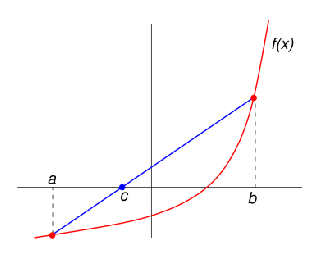
\epsfig{file=Figures/regula-falsi.eps,scale=1.0}
   \caption{Die Regula-Falsi zur Nullstellen-Bestimmung.}
  \label{fig:regula-falsi}
\end{figure}


Das Verfahren, das mit dieser Formel arbeitet, ist unter dem Namen 
\href{http://de.wikipedia.org/wiki/Regula_falsi}{\emph{Regula Falsi}}
bekannt und sieht genauso aus wie das Bisektions-Verfahren, nur dass wir f\"ur $c$ jetzt
die oben abgeleitete Formel verwenden:
\begin{enumerate}
\item[I.A.:] $n=1$.

      $a_1 := a$, \quad $b_1 := b$.
\item[I.S.:] $n \mapsto n+1$

      \hspace*{1.3cm} $c_n := \bruch{|f(b_n)|\cdot a_n + |f(a_n)|\cdot b_n}{|f(a_n)| + |f(b_n)|}$. \\[0.3cm]
      Dann definieren wir $a_{n+1}$ und $b_{n+1}$ durch Fall-Unterscheidung:
      \\[0.2cm]
      \hspace*{1.3cm}
      $\pair(a_{n+1},b_{n+1}) := 
         \left\{ \begin{array}{ll}
                 \pair(a_n,c_n) & \mbox{falls}\quad f(c_n) >    0 \\
                 \pair(c_n,b_n) & \mbox{falls}\quad f(c_n) \leq 0. \\
                 \end{array}
         \right.
      $
\end{enumerate}
\"Ahnlich wie beim Beweis des Zwischenwert-Satzes l\"asst sich zeigen, dass die Folge
$\folge{a_n}$ monoton steigend ist, w\"ahrend die Folge $\folge{b_n}$ monoton fallend ist.
Da die Folgen \"uberdies beschr\"ankt sind, denn $a_n$ ist immer kleiner als $b$ und $b_n$ ist
immer gr\"o{\ss}er als $a$, konvergieren beide Folgen.  Allerdings ist nicht garantiert, dass
$a_n$ und $b_n$ gegen den gleichen Grenzwert konvergieren!  Es l\"asst sich lediglich zeigen,
dass entweder $a_n$ oder $b_n$ gegen eine Nullstelle der Funktion $f$ konvergiert.
Um das Verfahren experimentell untersuchen zu k\"onnen, implementieren wir es.
Abbildung \ref{fig:regulaFalsi.stlx} zeigt die Implementierung der Methode
\textsl{findZero}().   Diese Implementierung ist weitgehend analog zu der Implementierung des
Bisektions-Verfahrens.  Es gibt eigentlich nur zwei wesentliche Unterschiede:
\begin{enumerate}
\item In Zeile 6 berechnen wir \texttt{c} nun nach der Formel
      \\[0.2cm]
      \hspace*{1.3cm}
      $\ds c := \bruch{f(b) \cdot a - f(a) \cdot b}{f(b) - f(a)}$. 
      \\[0.2cm]
      Beim Bisektions-Verfahren hatten wir hier die Formel
      \\[0.2cm]
      \hspace*{1.3cm}
      $\ds c := \frac{1}{2} \cdot (a + b)$
      \\[0.2cm]
      verwendet.
\item Bei der R\"uckgabe des berechneten Wertes in Zeile 14 bzw.~16 ist es erforderlich, die Betr\"age der
      Funktionswerte an den Intervall-Grenzen  \texttt{a} und \texttt{b} zu vergleichen, denn wir
      wissen nicht, ob die Folge $(a_n)_n$ oder die Folge $(b_n)_n$ gegen die Nullstelle von $f$
      konvergiert.  Wir geben daher als Ergebnis die 
      Intervall-Grenze  zur\"uck, f\"ur die der Betrag des Funktionswertes am kleinsten ist.
      Da wir wissen, dass der Funktionswert an der linken Intervall-Grenze immer kleiner als 0
      ist, erhalten wir dort den Betrag der Funktion $f$, indem wir dem Funktionswert das Minuszeichen
      vorstellen. 
\end{enumerate}

\begin{figure}[!ht]
  \centering
\begin{Verbatim}[ frame         = lines, 
                  framesep      = 0.3cm, 
                  labelposition = bottomline,
                  numbers       = left,
                  numbersep     = -0.2cm,
                  xleftmargin   = 0.5cm,
                  xrightmargin  = 0.5cm,
                ]
    regulaFalsi := procedure(f, a, b, n) {
        assert(a < b, "Error: !(a < b)");
        assert(f(a) < 0 && f(b) > 0, "Error: !(f(a) < 0 && f(b) > 0)");
        fa := f(a); fb := f(b); 
        for (i in [1 .. n]) {
            c  := (fb * a - fa * b) / (fb - fa); fc := f(c); 
            if (fc <= 0) {
                a := c; fa := fc; 
            } else {
                b := c; fb := fc; 
            }
        }
        if (-fa < fb) {
            return a;
        } else {
            return b;
        }
    };
\end{Verbatim}
\vspace*{-0.3cm}
  \caption{Implementierung der Regula Falsi in \textsc{SetlX}.}
  \label{fig:regulaFalsi.stlx}
\end{figure} %\$

Tabelle \ref{tab:regula-falsi} zeigt die ersten 12 Iterations-Schritte, wenn die Regula Falsi
zur Berechnung der Nullstelle von $x  - \cos(x)$ eingesetzt wird.  Wir sehen,
dass wir bereits im 9-ten Schritt dieselbe Genauigkeit erreicht haben, f\"ur die wir mit
dem Bisektions-Verfahren 30 Schritte ben\"otigt haben.  Wir sehen auch, dass die rechte
Intervall-Grenze immer konstant bleibt.  Es sieht so aus, als ob wir mit der Regula Falsi
ein Verfahren gefunden h\"atten, dass dem Bisektions-Verfahren \"uberlegen w\"are.  Die n\"achste Aufgabe
zeigt Ihnen jedoch, dass dem Verfahren eine ganz wichtige Eigenschaft fehlt, die das
Bisektions-Verfahren besitzt:  
\\[0.2cm]
\hspace*{0.3cm}
\colorbox{red}{\framebox{\colorbox{orange}{Das Verfahren, das die Regula Falsi zur Bestimmung der Nullstelle verwendet, ist nicht robust!}}}
\\[0.2cm]
Es gibt n\"amlich Funktionen, bei denen die Regula Falsi zur Nullstellen-Bestimmung
\textbf{\underline{wesentlich mehr}} Iterationen ben\"otigt als das Bisektions-Verfahren.
\vspace*{0.3cm}

\begin{table}[!h]
  \centering
\framebox{
  \begin{tabular}{|r|c|c|c|c|}
\hline
   $n$ & $a_n$ & $b_n$ & $f(a_n)$ & $f(b_n)$ \\
\hline
\hline
  1: & 0.000000000 & 1.000000000 & -1.00000000e+00 & 4.59697694e-01 \\ 
\hline
  2: & 0.685073357 & 1.000000000 & -8.92992765e-02 & 4.59697694e-01 \\ 
\hline
  3: & 0.736298997 & 1.000000000 & -4.66003904e-03 & 4.59697694e-01 \\ 
\hline
  4: & 0.738945356 & 1.000000000 & -2.33925666e-04 & 4.59697694e-01 \\ 
\hline
  5: & 0.739078130 & 1.000000000 & -1.17191742e-05 & 4.59697694e-01 \\ 
\hline
  6: & 0.739084782 & 1.000000000 & -5.87046549e-07 & 4.59697694e-01 \\ 
\hline
  7: & 0.739085115 & 1.000000000 & -2.94066726e-08 & 4.59697694e-01 \\ 
\hline
  8: & 0.739085132 & 1.000000000 & -1.47305551e-09 & 4.59697694e-01 \\ 
\hline
  9: & 0.739085133 & 1.000000000 & -7.37890543e-11 & 4.59697694e-01 \\ 
\hline
 10: & 0.739085133 & 1.000000000 & -3.69623245e-12 & 4.59697694e-01 \\ 
\hline
 11: & 0.739085133 & 1.000000000 & -1.85199566e-13 & 4.59697694e-01 \\ 
\hline
 12: & 0.739085133 & 1.000000000 & -9.23913723e-15 & 4.59697694e-01 \\ 
\hline
  \end{tabular}}
  \caption{Die ersten 12 Schritte der Regula Falsi zur L\"osung von $x - \cos(x) = 0$.}
  \label{tab:regula-falsi}
\end{table}


\exercise
 Verwenden Sie die Regula Falsi zur L\"osung der Gleichung 
\\[0.2cm]
\hspace*{1.3cm}
$x^4 - 1 = 0$.
\\[0.2cm]
Starten Sie mit dem Intervall $[0, 10]$. Zeigen Sie, dass f\"ur alle nat\"urlichen Zahlen $n$
mit $n \leq 1000$ die folgende Ungleichung f\"ur die linke Intervall-Grenze $a_n$ gilt:
\\[0.2cm]
\hspace*{1.3cm} $a_n \leq \bruch{n}{1000}$.
\\[0.2cm]
Die L\"osung der Gleichung $x^4 - 1 = 0$ in dem Intervall ist $x=1$.  Aus der zu zeigenden
Ungleichung kann beispielsweise gefolgert werden, dass $a_{100} \leq 0.1$ gilt.  
 Der mit dem obigen Programm ermittelte Wert f\"ur $a_{100}$ ist
$a_{100} = 0.0985146583$.  In diesem Fall hat die Regula Falsi also selbst nach  100
Iterationen nicht eine einzige korrekte Stelle 
im Ergebnis berechnen k\"onnen!  \eox
\vspace*{0.3cm}

\noindent
\textbf{L\"osung}: Wir zeigen durch vollst\"andige Induktion \"uber $n$, dass f\"ur alle 
$n\leq 1000$ zum einen die Ungleichung $a_n \leq n \cdot 10^{-3}$ gilt und dass zum anderen 
$b_n$ konstant ist, es gilt $b_n = 10$.
\begin{enumerate}
\item[I.A.:] $n = 1$.  Es gilt
      \\[0.2cm]
      \hspace*{1.3cm} $a_1 = 0 \leq 1 \cdot 10^{-3}$ \quad und \quad $b_1 = 10$.
\item[I.S.:] $n \mapsto n + 1$.

      Die Funktion $f := (x \mapsto x^4 - 1)$ ist f\"ur nicht-negative Zahlen \emph{monoton steigend},
      dass hei{\ss}t aus $0 \leq u \leq v$ folgt auch $f(u) \leq f(v)$.  Es gilt 
      \\[0.2cm]
      \hspace*{1.3cm}
      $f(n \cdot 10^{-3}) = n^4 \cdot 10^{-12} - 1$ \quad und \quad $f(10) = 10^4 - 1$.
      \\[0.2cm]
      Nach Induktions-Voraussetzung k\"onnen wir $a_n$ durch $n\cdot 10^{-3}$ nach oben absch\"atzen und 
      aufgrund der Monotonie von $f$ k\"onnen wir dann $f(a_n)$ durch $f(n\cdot 10^{-3})$ nach oben
      absch\"atzen:
      \\[0.2cm]
      \hspace*{1.3cm}
      $f(a_n) \leq f(n \cdot 10^{-3}) = n^4 \cdot 10^{-12} - 1$
      \\[0.2cm]
      Wenden wir daher f\"ur $a_n' = n \cdot 10^{-3}$ und $b_n=10$ die Regula Falsi an um eine
      N\"aherung $c_n'$ f\"ur die Nullstelle von $f$ zu berechnen, so wird
      $c_n'$ gr\"o{\ss}er sein als der wahre Wert von $c_n$, der in dem Algorithmus tats\"achlich auftritt.
      Es gilt:
      \\[0.2cm]
      \hspace*{1.3cm}
    $
    \begin{array}[t]{lcl}
    c_n' & = & \bruch{f(b_n) \cdot a_n' - f(a_n') \cdot b_n}{f(b_n) - f(a_n')} \\[0.5cm]
      & = & \bruch{f(10) \cdot n \cdot 10^{-3} - f\bigl(n\cdot 10^{-3}\bigr) \cdot 10}{f(10) - f\bigl(n\cdot 10^{-3}\bigr)} \\[0.5cm]
      & = & \bruch{\bigl(10^4 - 1\bigr) \cdot n \cdot 10^{-3} - \bigl(n^4 \cdot 10^{-12} - 1\bigr)\cdot 10}{10^4 - 1 - n^4\cdot 10^{-12} + 1} \\[0.5cm]
      & = & 10^{-4}\cdot \bruch{10 \cdot n - n \cdot 10^{-3} - n^4 \cdot 10^{-11} + 10}{1 - n^4\cdot 10^{-16}} \\[0.5cm]
      & = & 10^{-3}\cdot \bruch{n + 1 - n \cdot 10^{-4} - n^4 \cdot 10^{-12}}{1 - n^4\cdot 10^{-16}} \\[0.5cm]
    \end{array}  
    $
      \\[0.2cm]
      Wir untersuchen nun, f\"ur welche nat\"urlichen Zahlen $n$ die Ungleichung 
      $c_n' \leq 10^{-3}\cdot (n+1)$ gilt.
      \\[0.2cm]
      \hspace*{1.3cm}
      $
      \begin{array}[t]{ll}        
                        & c_n' \leq 10^{-3}\cdot (n+1) \\[0.2cm]
        \Leftrightarrow & 10^{-3}\cdot \bruch{n + 1 - n \cdot 10^{-4} - n^4 \cdot 10^{-12}}{1 - n^4\cdot 10^{-16}} \leq 10^{-3}\cdot (n+1) \\[0.5cm]
        \Leftrightarrow & n + 1 - n \cdot 10^{-4} - n^4 \cdot 10^{-12} \leq (n+1)\cdot \bigl(1 - n^4\cdot 10^{-16}\bigr)   \\[0.3cm]
        \Leftrightarrow & n + 1 - n \cdot 10^{-4} - n^4 \cdot 10^{-12} \leq (n+1)  - (n+1)\cdot n^4\cdot 10^{-16}   \\[0.3cm]
        \Leftrightarrow & - n \cdot 10^{-4} - n^4 \cdot 10^{-12} \leq   - (n+1)\cdot n^4\cdot 10^{-16}   \\[0.3cm]
        \Leftrightarrow & n \cdot 10^{-4} + n^4 \cdot 10^{-12} \geq  (n+1)\cdot n^4\cdot 10^{-16}   \\[0.3cm]
        \Leftarrow      & n^4 \cdot 10^{-12} \geq  (n+1)\cdot n^4\cdot 10^{-16}   \\[0.3cm]
        \Leftrightarrow & 1 \geq  (n+1)\cdot 10^{-4}   \\[0.3cm]
        \Leftrightarrow & 10^4 \geq  n+1   \\[0.3cm]
        \Leftrightarrow & n \leq 9999   
      \end{array}
      $
      \\[0.3cm]
      Solange $n < 1000$ ist, gilt also sicher $c_n' < 1$ und damit ist $f(c_n')$ negativ.
      Daher gilt 
      \\[0.2cm]
      \hspace*{1.3cm}  $a_{n+1} \leq a_{n+1}' = c_n' \leq 10^{-3} \cdot n < 10^{-3} \cdot (n+1)$ und $b_{n+1} = b_n = 10$.
      \qed
\end{enumerate}

\subsection{Das Sekanten-Verfahren}
Ein Problem bei der Regula Falsi scheint darin zu liegen, dass h\"aufig eine
Intervall-Grenze w\"ahrend der gesamten Iteration fest bleibt.  Dies war schon bei der
Bestimmung der Nullstelle der Funktion
\\[0.2cm]
\hspace*{1.3cm}
$x \mapsto x - \cos(x)$ 
\\[0.2cm]
der Fall.  Eine
M\"oglichkeit, dieses Problem zu umgehen besteht darin, dass wir anstatt eine Folge von
Intervallen $\folge{[a_n, b_n]}$ zu bilden, einfach nur eine Folge von Punkten
$\folge{x_n}$ konstruieren.  Den Punkt $x_{n+1}$ bestimmen wir, indem wir durch die Punkte
$x_{n+1}$ und $x_n$ eine Gerade legen und dann $x_n$ als den Schnittpunkt dieser Geraden
mit der $x$-Achse bestimmen.  Das f\"uhrt auf dieselbe Formel wie bei der Regula-Falsi, wir
setzen n\"amlich
\\[0.2cm]
\hspace*{1.3cm}
$x_{n+1} := \bruch{f(x_{n}) \cdot x_{n-1} - f(x_{n-1}) \cdot x_n}{f(x_{n}) - f(x_{n-1})}$.
\\[0.2cm]
Dann brauchen wir nur noch zwei Startwerte $x_1$ und $x_2$ und die Rechnung kann los gehen.
Abbildung \ref{fig:secant.stlx} zeigt eine Implementierung des Sekanten-Verfahrens in
\textsc{SetlX}.  Testen wir dieses Programm mit der Funktion $x \mapsto x - \cos(x)$, so
erhalten wir die in Tabelle \ref{tab:secant-method} gezeigten Werte.
Wir sehen, dass jetzt bereits 7 Iterationen ausreichen, um die L\"osung der Gleichung mit
der geforderten Genauigkeit zu berechnen.  Es sieht also so aus, als ob das
Sekanten-Verfahren den anderen Verfahren \"uberlegen ist.  In der Tat kann gezeigt werden, dass
das Sekanten-Verfahren, \textbf{wenn} es denn konvergiert, schneller konvergiert als die anderen
Verfahren. Wir werden das sp\"ater pr\"azisieren.  Das Problem ist, dass das Sekanten-Verfahren
gar nicht immer konvergiert.  Betrachten wir beispielsweise die Funktion 
\\[0.2cm]
\hspace*{1.3cm}
$x \mapsto \bruch{2}{x^2 + 1} - 1$. 
\\[0.2cm]
Diese Funktion hat bei $x = 1.0$ eine Nullstelle.  Mit
den Startwerten $a = 0$ und $b = 5.0$ produziert unser Programm die in Tabelle
\ref{tab:secant-method2}
gezeigten Werte.


\begin{figure}[!ht]
  \centering
\begin{Verbatim}[ frame         = lines, 
                  framesep      = 0.3cm, 
                  labelposition = bottomline,
                  numbers       = left,
                  numbersep     = -0.2cm,
                  xleftmargin   = 0.5cm,
                  xrightmargin  = 0.5cm,
                ]
    secant := procedure(f, a, b, digits) {
        fa := f(a); 
        fb := f(b); 
        while (abs(b - a) > (1/10)**(digits + 1)) {
            c := (fb * a - fa * b) / (fb - fa);
            a := b; b := c; fa := fb; fb := f(c); 
        }
        return b;
    };
\end{Verbatim}
\vspace*{-0.3cm}
  \caption{Implementierung des Sekanten-Verfahrens in \textsc{SetlX}.}
  \label{fig:secant.stlx}
\end{figure} %\$


\begin{table}[!h]
  \centering
\framebox{
  \begin{tabular}{|r|r|r|}
\hline
   $n$ & $x_n$ & $f(x_n)$ \\
\hline
\hline
  1: & \texttt{10.00000000000} & \texttt{+1.08390715e+01} \\
\hline
  2: & \texttt{ 0.84466083134} & \texttt{+1.80675899e-01} \\
\hline
  3: & \texttt{ 0.68946400911} & \texttt{-8.21230732e-02} \\
\hline
  4: & \texttt{ 0.73796206792} & \texttt{-1.87910933e-03} \\
\hline
  5: & \texttt{ 0.73909776898} & \texttt{+2.11474296e-05} \\
\hline
  6: & \texttt{ 0.73908513008} & \texttt{-5.24715686e-09} \\
\hline
  7: & \texttt{ 0.73908513322} & \texttt{-1.46275678e-14} \\
\hline
  \end{tabular}}
  \caption{L\"osung der Gleichung $x - \cos(x) = 0$ mit dem Sekanten-Verfahren.}
  \label{tab:secant-method}
\end{table}



\begin{table}[!h]
  \centering
\framebox{
  \begin{tabular}{|r|r|r|}
\hline
   $n$ & $x_n$ & $f(x_n)$ \\
\hline
\hline
  1: & \texttt{+5.000000e+00} & \texttt{-0.923076923} \\
\hline
  2: & \texttt{+2.600000e+00} & \texttt{-0.742268041} \\
\hline
  3: & \texttt{-7.252631e+00} & \texttt{-0.962687030} \\
\hline
  4: & \texttt{+3.577905e+01} & \texttt{-0.998438891}\\
\hline
  5: & \texttt{-1.165962e+03} & \texttt{-0.999998529}\\
\hline
  6: & \texttt{+7.693592e+05} & \texttt{-1.000000000}\\
\hline
  7: & \texttt{-5.237534e+11} & \texttt{-1.000000000}\\
\hline
  8: & \texttt{+1.550094e+23} & \texttt{-1.000000000}\\
\hline
  9: & $\infty$               & \texttt{-1.000000000}\\
\hline
  \end{tabular}}
  \caption{Divergenz des Sekanten-Verfahrens bei der L\"osung von $\bruch{2}{x^2 + 1} - 1 = 0$.}
  \label{tab:secant-method2}
\end{table}





\subsection{Das Illinois-Verfahren}
Von den bisher vorgestellten Verfahren ist nur das Bisektions-Verfahren wirklich robust.
Bei der Regula-Falsi ist das Problem, dass eine Intervall-Grenze stehen bleiben kann. Am
Beispiel der Funktion
\\[0.2cm]
\hspace*{1.3cm}
 $x \mapsto x^4 - 1$ 
\\[0.2cm]
haben wir gesehen, dass dies zu einer sehr
langsamen Konvergenz f\"uhren kann.  Beim Sekanten-Verfahren hatten wir dieses Problem
behoben, aber dort kann es in ung\"unstigen F\"allen passieren, dass das Verfahren \"uberhaupt nicht mehr
konvergiert.  Das \emph{Illinois-Verfahren} \cite{dowell:1971} versucht die Konvergenz der Regula Falsi
auf andere Weise zu beschleunigen.  Die Idee des Verfahrens ist eigentlich sehr naheliegend:
Wenn bei der Regula Falsi eine der Intervall-Grenzen \"uber zwei oder mehr Schritte konstant bleibt,
dann wird der Funktionswert an der betreffenden Intervall-Grenze halbiert, so dass der Einfluss dieses
Wertes bei der Berechnung der n\"achsten N\"aherung $c_n$ nach der Formel
\\[0.2cm]
\hspace*{1.3cm}
$c_n := \bruch{f(b_n) \cdot a_n - f(a_n) \cdot b_n}{f(b_n) - f(a_n)}$
\\[0.2cm]
gemindert wird.  Nehmen wir o.B.d.A.~an, dass $f(a) < 0$ und $0 < f(b)$ ist, so f\"uhrt das zur folgenden 
Definition der Folgen $\folge{a_n}$ und $\folge{b_n}$:
\begin{enumerate}
\item[I.A.:] $n=1$.  Wir setzen 
             \\[0.2cm]
             \hspace*{1.3cm}
             $a_1 := a$, \quad $b_1 := b$, \quad $\alpha_1 := 1$, \quad und \quad $\beta_1 := 1$.
             \\[0.2cm]
             Die Werte $\alpha_1$ und $\beta_1$ sind dabei Gewichtungs-Faktoren, die wir sp\"ater ben\"otigen.
\item[I.S.:] $n \mapsto n+1$.  Wir definieren \"ahnlich wie bei der Regula Falsi den Wert $c_n$ als \\[0.2cm]
      \hspace*{1.3cm} 
      $c_n := \bruch{\beta_n \cdot f(b_n) \cdot a_n - \alpha_n \cdot f(a_n) \cdot b_n}{
                     \beta_n \cdot f(b_n) - \alpha_n \cdot f(a_n)}
      $. 
      \\[0.3cm]
      Der Unterschied zur Regula Falsi liegt in den Gewichtungs-Faktoren $\alpha_n$ und $\beta_n$.
      Die Werte f\"ur $a_{n+1}$ und $b_{n+1}$ werden durch dieselbe Fall-Unterscheidung wie bei der Regula
      Falsi festgelegt:
      \\[0.2cm]
      \hspace*{1.3cm}
      $\pair(a_{n+1},b_{n+1}) := 
         \left\{ \begin{array}{ll}
                 \pair(a_n,c_n) & \mbox{falls}\quad f(c_n) >    0 \\
                 \pair(c_n,b_n) & \mbox{falls}\quad f(c_n) \leq 0. \\
                 \end{array}
         \right.
      $
      \\[0.2cm]
      Falls wir nun feststellen, dass $b_{n+1} = b_{n-1}$ ist, so hat sich der Wert der rechten
      Intervall-Grenze w\"ahrend der letzten zwei Iterationen nicht ge\"andert.  Wir wollen diesen Wert
      daher beim n\"achsten Iterations-Schritt 
      schw\"acher gewichten und setzen deshalb in diesem Fall
      \\[0.2cm]
      \hspace*{1.3cm}
      $\beta_{n+1} := \bruch{1}{2} \cdot \beta_n$ \quad und \quad $\alpha_{n+1} := 1$.
      \\[0.2cm]
      Ist umgekehrt $a_{n+1} = a_{n-1}$, so hat sich der Wert der linken
      Intervall-Grenze nicht ge\"andert.  Wir gewichten daher die linke Intervall-Grenze beim n\"achsten
      Iterations-Schritt schw\"acher und setzen 
      \\[0.2cm]
      \hspace*{1.3cm}
      $\beta_{n+1} := 1$ \quad und \quad $\alpha_{n+1} := \bruch{1}{2} \cdot \alpha_n$.
      \\[0.2cm]
      In allen anderen F\"allen setzen wir 
      \\[0.2cm]
      \hspace*{1.3cm}
      $\beta_{n+1} := 1$ \quad und \quad $\alpha_{n+1} := 1$.
\end{enumerate}
Die Umsetzung dieses Verfahrens sehen Sie in Abbildung \ref{fig:illinois.stlx}.  In den Variablen
\texttt{oldA1} und \texttt{oldB1} speichern wir die Werte von $a_{n-1}$ und $b_{n-1}$, in den
Variablen \texttt{oldA2} und \texttt{oldB2} sind die Werte $a_{n-2}$ und $b_{n-2}$ gespeichert.  Wir
initialisieren diese Werte mit $\mathtt{om}$, denn $\mathtt{om}$ bezeichnet in \textsc{SetlX}
den undefinierten Wert.
Falls wir in Zeile 19 feststellen, dass der Wert von $a_n = a_{n-2}$ ist, dann setzen wir den Wert
$\alpha_{n+1}$ auf $\alpha_n/2$.  Analog testen wir in Zeile 14, ob $b_n = b_{n-2}$ ist und setzen
gegebenenfalls $\beta_{n+1}$ auf $\beta_n/2$.



\begin{figure}[!ht]
  \centering
\begin{Verbatim}[ frame         = lines, 
                  framesep      = 0.3cm, 
                  labelposition = bottomline,
                  numbers       = left,
                  numbersep     = -0.2cm,
                  xleftmargin   = 0.0cm,
                  xrightmargin  = 0.0cm,
                ]
    illinois := procedure(f, a, b, n) {
        assert(a < b, "a has to be less than b");
        assert(f(a) < 0 && 0 < f(b), "We need f(a) < 0 and 0 < f(b)!");
        [ fa, fb ] := [ f(a), f(b) ];
        oldA1 := om; oldB1 := om;
        oldA2 := om; oldB2 := om;
        alpha := 1; beta := 1;
        for (k in [1 .. n]) {
            c  := (beta * fb * a - alpha * fa * b) / (beta * fb - alpha * fa);
            fc := f(c);
            if (fc < 0) {
                a := c; fa := fc; alpha := 1;
                if (oldB2 == b) {
                    beta /= 2;
                }
            } else if (fc > 0) {
                b := c; fb := fc; beta := 1;
                if (oldA2 == a) {
                    alpha /= 2;
                }
            } else {
                return c;
            }
            oldA2 := oldA1; oldB2 := oldB1;
            oldA1 := a;     oldB1 := b;
        }
        return (a + b) / 2;
    };
\end{Verbatim}
\vspace*{-0.3cm}
  \caption{Implementierung des Illinois-Verfahrens zur Berechnung von Nullstellen.}
  \label{fig:illinois.stlx}
\end{figure} 

%%% Local Variables: 
%%% mode: latex
%%% TeX-master: "analysis"
%%% End: 
